\chapter{Result and discussion}

\AddToShipoutPictureBG*{%
  \AtPageUpperLeft{%
    \hspace*{18.25cm}%
    \raisebox{-3cm}{%
      \makebox[0pt][r]{\parbox{\textwidth}{\begin{flushright}\textit{``The distance between insanity and genius is measured only by success.''}\\
      Bruce Feirstein\end{flushright}}}
}}}%

We have applied the proposed methods to an urban microclimate system simulated by the UWG. In particular, the UWG model has been calibrated based on the urban outdoor air temperature in District E3 of downtown Abu Dhabi (UAE) during 2017. This chapter presents and discusses the main results.

\section{Overview}

The case study was conducted in District E3, the same area detailed in \textbf{Chapter 3}. The measured rural data from the Masdar Institute Field Station during calendar year 2017 is used for running the UWG. For the urban outdoor air temperature, we use the data measured in 2017 from all six of the same calibrated sensors that present consistent performances. The locations of these sensors are depicted as the red-cross points in \textbf{Figure 3-1(c)}. The temperature observations at 8.5 m were selected for validating the calibrated models.

In this study, we use the urban-rural outdoor air temperature difference to cali-brate the UWG. A good fit between the predicted and measured temperature trajectories is one indication that the model has captured the thermal dynamics well. Other calibration studies based on energy use instead of air temperature may increase the solution uncertainty, since various combinations of the system properties can easily produce similar consumptions. We also find that some researchers have used air temperature to analyze or calibrate building thermal simulations \cite{ruiz2016genetic,ruiz2017analysis,spitz2012practical,cornaro2015thermal}.

First, a Latin Hypercube sample matrix of size $N = 1000$ has been generated and propagated via the UWG for summer (August 1-7) and winter (February 1-7) in 2017, respectively. For each trial, the predicted hourly outdoor air temperatures were saved. The computation of a one-week scenario lasted around \textit{one minute} on a 3.00GHz processor computer for each trial. To the author's knowledge, this is to date the fastest simulation engine to estimate the microclimate conditions for a specific urban site using physics-based model setting. Finally, corresponding indices (i.e., SRC and R$^2$) were calculated based on the generated results to enable uncertainty and sensitivity analysis.

Once the weak parameters were identified according to some specified criteria, their values were set via MC filtering based on the information contained in those input vectors with the lowest GOFs. The strong parameters, on the other hand, were considered to be tuned in the subsequent EA-based optimization. The objective function used to guide the EA is the GOF based on weekly-average diurnal profiles of the urban-rural outdoor air temperature difference in February 1-7 and August 1-7, 2017. That is, we are calibrating the strong parameters only based on the measurements in one summer week and one winter week.

In order to evaluate the associated uncertainty as predicted by the calibrated solutions, we ran 10 independent trials for both the traditional and online hyper-heuristic EAs. All the trials used the same stop criteria: the evolution ends when the number of expensive evaluations exceeds the maximum 2040 or the evolution lasts more than 60 generations. The goal is to find the algorithm setup returning the lowest GOF for the same number of evaluations within fixed computation budgets (i.e., better quality solution given the same effort); this goal precluded use of a convergence criterion. Also provided were comparisons of the computational effort required to obtain the same quality of solutions. An internal cache of previously-evaluated solutions is maintained in the online hyper-heuristic EA for each run, to avoid re-evaluating the same solutions. The solutions drawn from the cache do not count toward the limit of 2040. Finally, the resulting solution sets from the 10 trials of the online hyper-heuristic EA were evaluated using the measurements.

\section{Uncertainty analysis}

The cumulative distribution functions are used to present the results from the Monte Carlo simulations and to display percentiles and confidence intervals of the outputs. \textbf{Figure 5-1} illustrates the uncertainty range of the weekly-average diurnal profile of the predicted outdoor air temperature in summer and winter, 2017. The shaded area represents the predicted values ranging from the 5th to 95th percentile, while the solid line represents the predicted value of the 50th percentile (i.e., median). It can be said that a model is robust enough to simulate the underlying phenomenon if, fed by the inputs with a given uncertainty, it is able to produce responses in a suitably small range. Thus, we can claim from \textbf{Figure 5-1} that the UWG is a fairly good simulator to approximate the thermal behavior of an urban microclimate system for different seasons with a specific degree of robustness. In addition, the results are quite consistent with those in our former study \cite{mao2017global} when we performed identical analysis on the same UWG model for summer and winter in 2016.

\begin{figure}[]
\centering
\includegraphics[width=.85\linewidth]{Figure5-1.eps}
\caption{Uncertainty range of the weekly-average diurnal profiles of the predicted urban outdoor air temperature based on Monte Carlo sampling: (a) Results between August 1 and 7, 2017 (summer); (b) Results between February 1 and 7, 2017 (winter). The shaded area represents the predicted values ranging from the 5th to 95th percentile. The solid line represents the predicted values of the 50th percentile.}
\end{figure}

It is interesting to observe that both the predicted summer uncertainty band and diurnal variation are generally larger than the winter ones. A possible reason lies in the seasonal variation of cooling load and solar radiation. During the summer in Abu Dhabi, the cooling demand and solar radiation become very high, resulting in a situation where the HVAC- and radiation-related parameters may have relatively larger impacts on the variation of the microclimate. During the winter, however, the role of these parameters in the urban thermal process becomes quite trivial.

\section{Sensitivity analysis}

Based on the evaluations with a large sample size, it seems reasonable to state that 0.025 (2.5\%) is a sufficient threshold for obtaining good SRC values \cite{saltelli2004sensitivity,menberg2016sensitivity}. Thus we decide that, for the present study, the parameter with an average of the absolute SRCs larger than 2.5\% over 24 hours in one day should have a significant impact on the model output. The resulting hourly coefficients of determination (R$^2$) are summarized in \textbf{Table 5.1}. The generally high R$^2$ values for most hours suggest that the higher-order effects due to non-linear behavior or parameter interaction play a fairly trivial role in the current model setting. This increases our confidence of using the SRC for the sensitivity analysis, which then identified 10 significant parameters for summer and eight for winter in 2017. \textbf{Figures 5-2 and 5-3} plot their hourly SRCs for each group respectively. The results are very consistent with those in our former study \cite{mao2017global} when we performed identical analysis on the same UWG model for summer and winter in 2016.

\begin{table}[]
\footnotesize
\centering
\caption{Coefficient of determination (R$^2$) of the regression model for the weekly-average diurnal profiles of the predicted urban outdoor air temperature during 2017.}
\begin{tabular}{lllllll}
\toprule
Hour & Summer & Winter &  & Hour & Summer & Winter \\ \hline
1    & 0.734  & 0.815  &  & 13   & 0.825  & 0.787  \\
2    & 0.712  & 0.810  &  & 14   & 0.797  & 0.778  \\
3    & 0.735  & 0.830  &  & 15   & 0.701  & 0.760  \\
4    & 0.778  & 0.797  &  & 16   & 0.745  & 0.741  \\
5    & 0.756  & 0.841  &  & 17   & 0.790  & 0.721  \\
6    & 0.815  & 0.855  &  & 18   & 0.796  & 0.738  \\
7    & 0.772  & 0.825  &  & 19   & 0.789  & 0.779  \\
8    & 0.782  & 0.818  &  & 20   & 0.751  & 0.761  \\
9    & 0.790  & 0.810  &  & 21   & 0.772  & 0.771  \\
10   & 0.731  & 0.768  &  & 22   & 0.718  & 0.783  \\
11   & 0.798  & 0.755  &  & 23   & 0.779  & 0.795  \\
12   & 0.837  & 0.783  &  & 24   & 0.770  & 0.807  \\
\bottomrule
\end{tabular}
\end{table}

\begin{figure}[h]
\centering
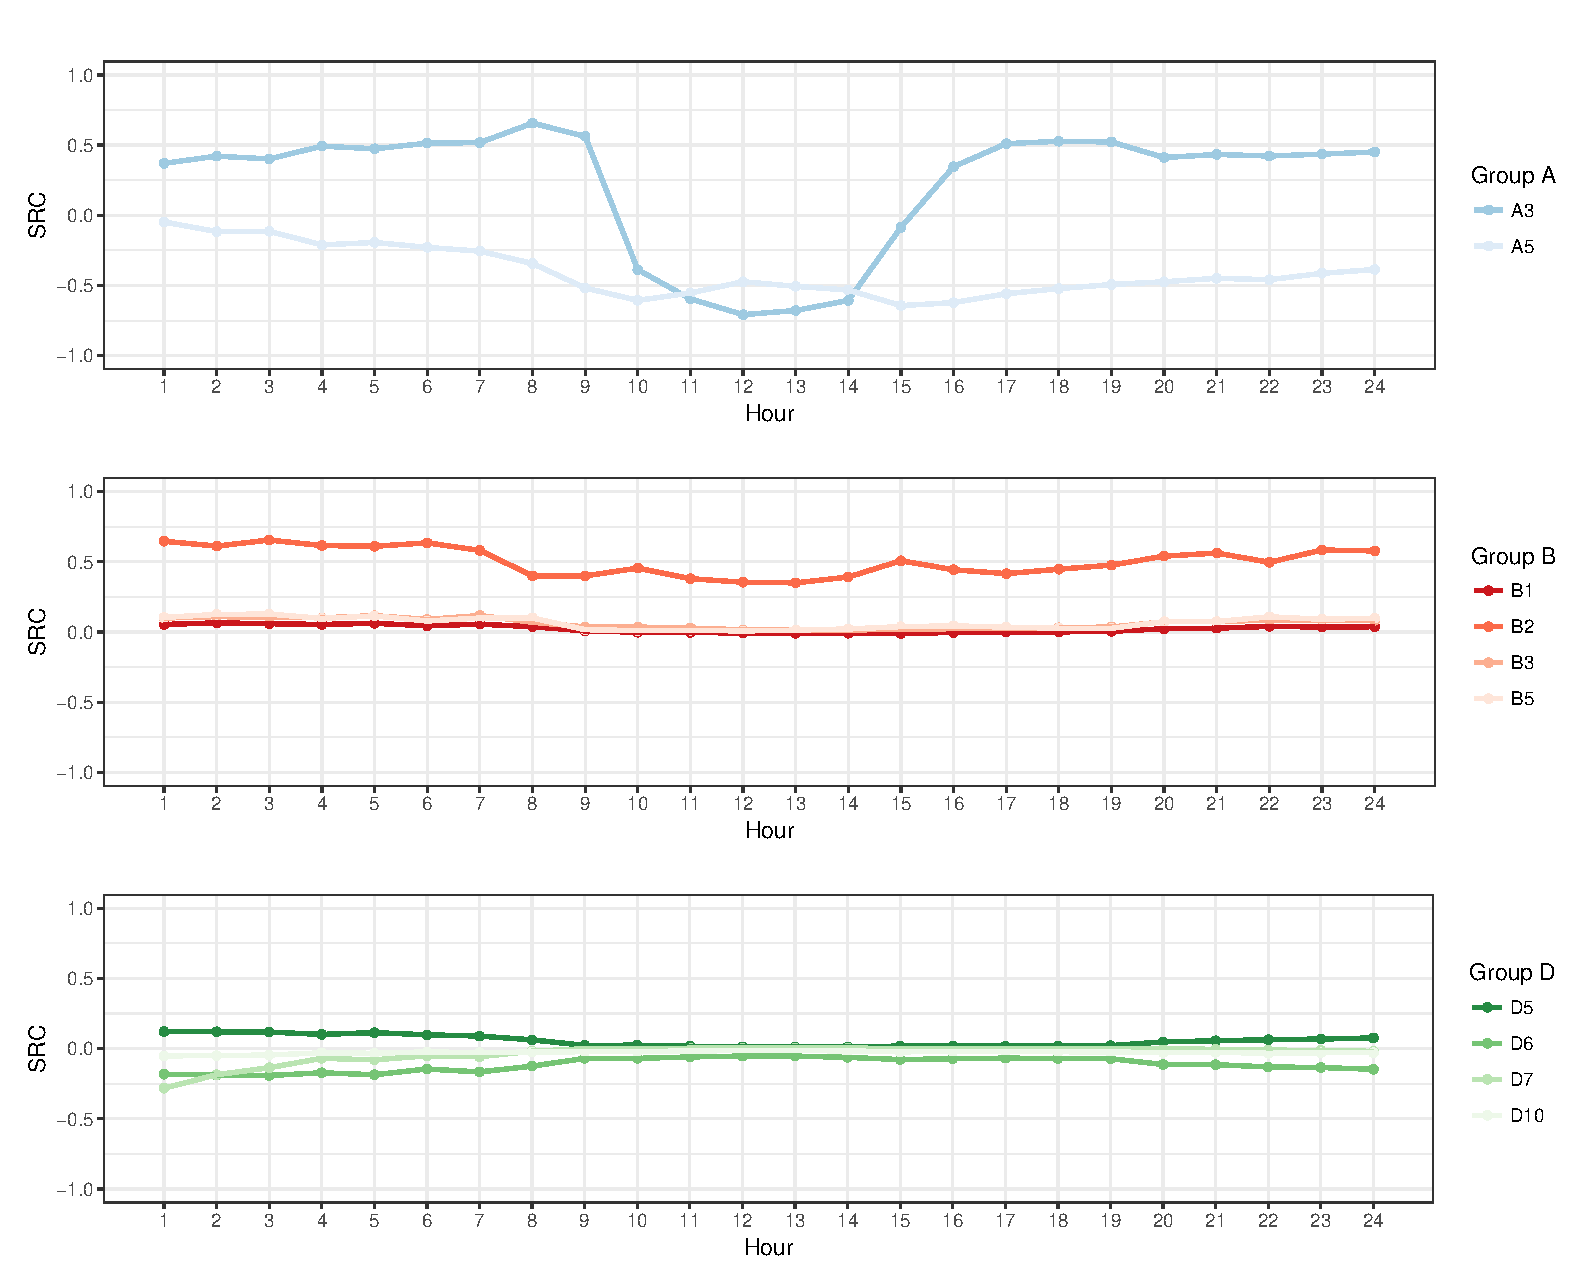
\includegraphics[width=.875\linewidth]{Figure5-2.eps}
\caption{The significant parameters obtained from the global sensitivity analysis of the weekly-average diurnal profiles of the predicted urban outdoor air temperature between August 1 and 7, 2017 (summer). The parameter denotations are the same as those defined in \textbf{Table 4.1}.}
\end{figure}

\begin{figure}[h]
\centering
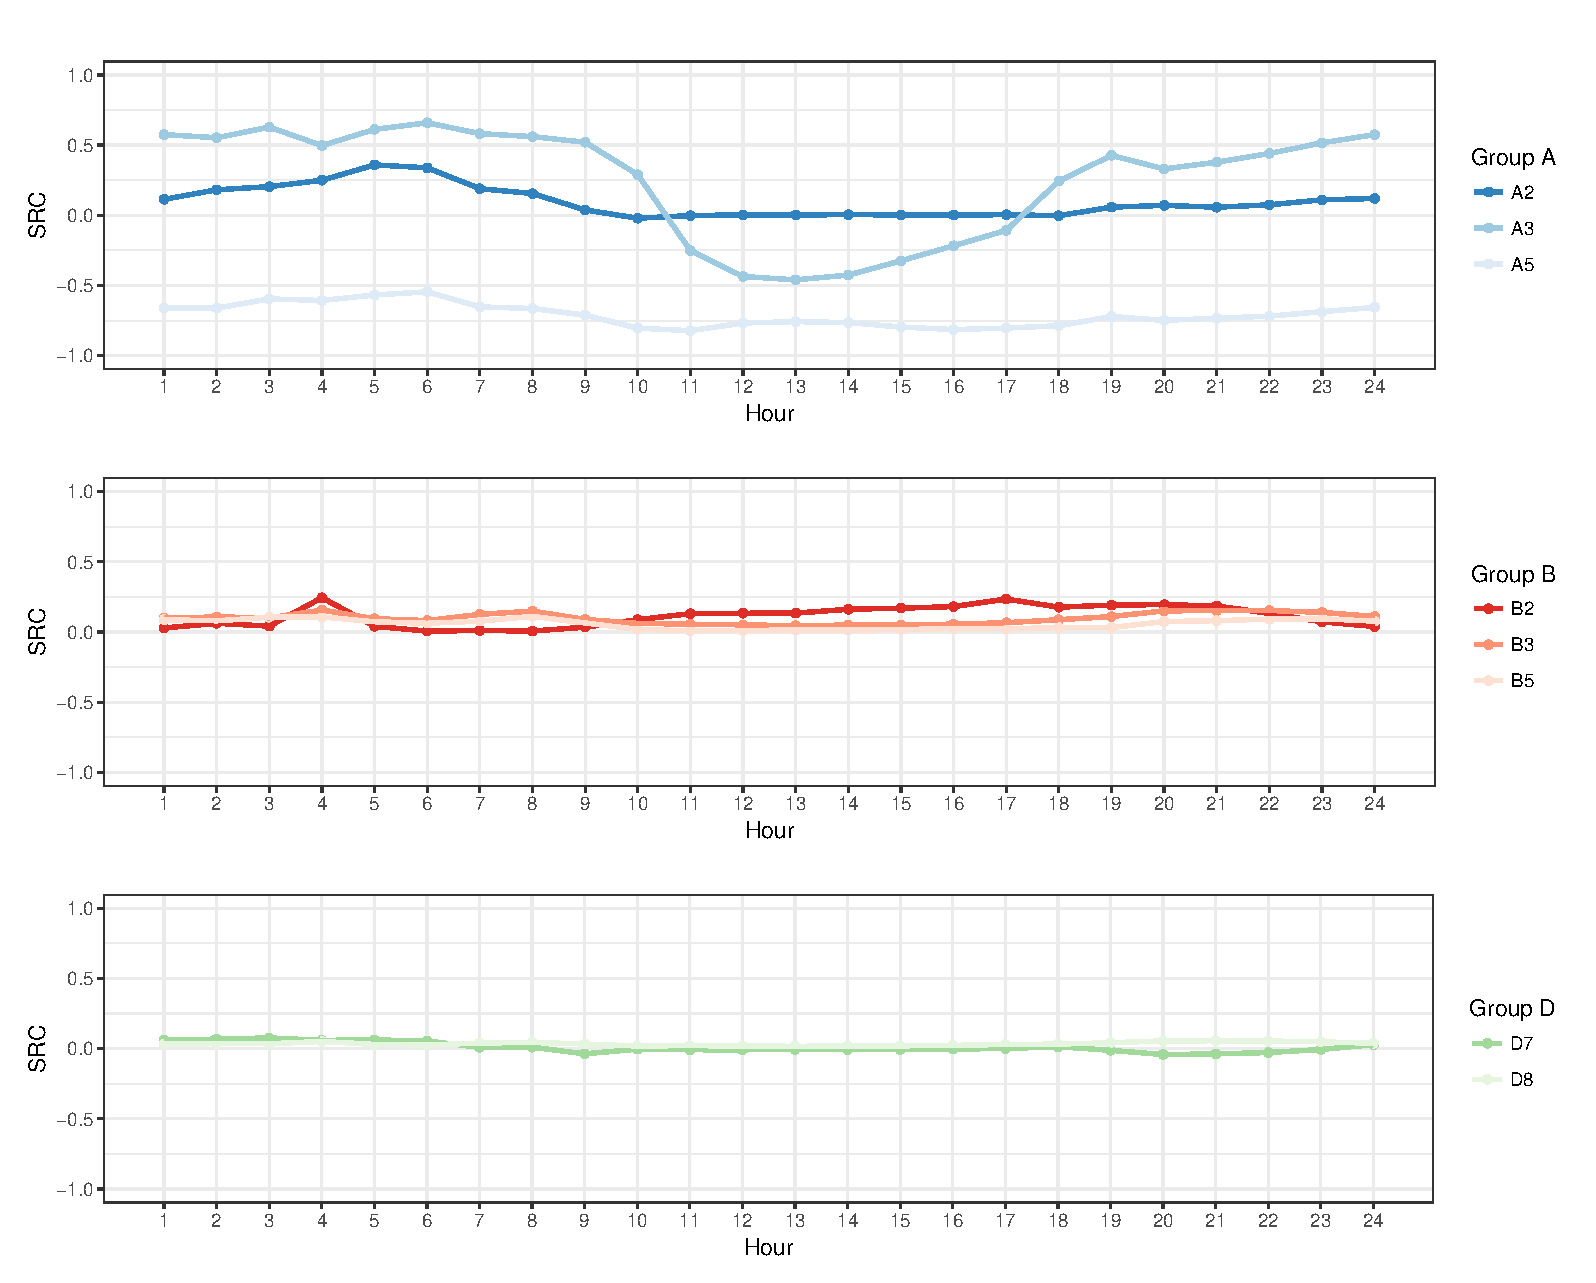
\includegraphics[width=.875\linewidth]{Figure5-3.eps}
\caption{The significant parameters obtained from the global sensitivity analysis of the weekly-average diurnal profiles of the predicted urban outdoor air temperature between February 1 and 7, 2017 (winter). The parameter denotations are the same as those defined in \textbf{Table 4.1}.}
\end{figure}

It is important to mention that no parameter in Group C (vegetation variables) is identified as a strong parameter. This can be explained by the fact that there is nearly no vegetation in Abu Dhabi, thus resulting in relatively smaller uncertainty ranges for the vegetation coverages (see \textbf{Table 4.1}). Previously, Bueno et al. \cite{bueno2013urban} reported that the case study of Basel (Switzerland) is sensitive to some vegetation parameters. We should emphasize that the UHI effect seems to vary locally from one place to another and thus the parameter sensitivity needs to be considered case by case.

It can also be seen from \textbf{Figures 5-2 and 5-3} that although all the parameters have an impact, the most critical ones are the reference height of the VDM (A3), the UCM-UBL exchange coefficient (A5), the fraction of waste heat into canyon (B2), and the nighttime urban boundary layer height (A2, for winter only). Ironically, these parameters remain the most uncertain among all the input variables. The reference height of the VDM and the nighttime urban boundary layer height are obtained from previous mesoscale atmospheric simulations \cite{li2013multi,hidalgo2008urban} because no observations are available. The UCM-UBL exchange coefficient and the fraction of waste heat into canyon are derived from the previous literature \cite{hanna2010wind} and well-educated guesses with limited domain knowledge. Since an urban system is typically characterized by a multiplicity of dynamic (building), stochastic (occupant), and probabilistic (weather) elements, it is difficult to find the exact values for these parameters for a given urban site. In order to capture the site-specific microclimate effects and reduce the uncertainty in the UWG model, additional numerical simulations of the established energy balances might be required. In addition, future improvement of the assessment would be to conduct more detailed estimate of higher-order effects, thus revealing deeper insights into the complex parameter behavior.

Finally, the difference between the summer and winter case suggests that we should focus on different parameters when studying different periods of time. Nevertheless, the identified key factors will be the subject of our subsequent research on the urban microclimate system in Abu Dhabi.

\section{Performance of the Monte Carlo filtering}

\begin{table}[!h]
\footnotesize
\begin{center}
\caption{List of the strong and weak parameters from the Monte Carlo filtering.}
\begin{tabular}{lll}
\toprule
Strong parameter                                  & Unit        & Range            \\ \hline
Nighttime urban boundary layer height (A2)        & m           & {[}50, 100{]}    \\
Reference height of the VDM (A3)                  & m           & {[}100, 200{]}   \\
UCM-UBL exchange coefficient (A5)                 & -           & {[}0.1, 0.9{]}   \\
Average building height (B1)                      & m           & {[}30, 40{]}     \\
Fraction of waste heat into canyon (B2)           & -           & {[}0.1, 0.9{]}   \\
Building density (B3)                             & -           & {[}0.15, 0.35{]} \\
Urban area characteristic length (B5)             & m           & {[}800, 1200{]}  \\
Infiltration rate (D5)                            & ACH         & {[}0.1, 0.7{]}   \\
Chiller COP (D6)                                  & -           & {[}2, 4{]}       \\
Indoor air temperature set point (D7)             & $^{\circ}$C          & {[}20, 24{]}     \\
Equipment load density (D8)                       & W m$^{-2}$       & {[}10, 16{]}     \\
Occupancy density (D10)                           & m$^2$ person$^{-1}$ & {[}15, 25{]}     \\ \hline
\rule{0pt}{2.75ex}Weak parameter                                    & Unit        & Value            \\ \hline
Daytime urban boundary layer height (A1)          & m           & 753.31           \\
Circulation coefficient (A4)                      & -           & 0.98             \\
Heat flux threshold for daytime conditions (A6)   & W m$^{-2}$       & 199.04           \\
Heat flux threshold for nighttime conditions (A7) & W m$^{-2}$       & 50.59            \\
Vertical-to-horizontal ratio (B4)                 & -           & 2.19             \\
Road albedo (B6)                                  & -           & 0.16             \\
Traffic sensible anthropogenic heat (peak) (B7)   & W m$^{-2}$       & 20.35            \\
Urban grass coverage (C1)                         & -           & 0.04             \\
Urban tree coverage (C2)                          & -           & 0.04             \\
Vegetation albedo (C3)                            & -           & 0.25             \\
Latent fraction of grass (C4)                     & -           & 0.61             \\
Latent fraction of tree (C5)                      & -           & 0.70             \\
Rural vegetation coverage (C6)                    & -           & 0.04             \\
Glazing ratio (D1)                                & -           & 0.50             \\
Wall U-value (D2)                                 & W m$^{-2}$ K$^{-1}$   & 2.52             \\
Window U-value (D3)                               & W m$^{-2}$ K$^{-1}$   & 3.18             \\
Window SHGC (D4)                                  & -           & 0.60             \\
Lighting load density (D9)                        & W m$^{-2}$       & 9.90             \\
\bottomrule
\end{tabular}
\end{center}
Note: \\
(a) The values of the weak parameters are set using the average of the top 20 promising input vectors in terms of the GOF. \\
(b) The identified strong parameters along with the associated ranges will be adjusted through an EA-based calibration process.
\end{table}

Given the results of SA, the weak parameters were then removed from the subsequent calibration process. Their static values were determined, somewhat arbitrarily, using the average of the 20 input vectors with the lowest GOFs. In addition, many strong parameters may have associated higher uncertainties and perhaps be more likely in need of tweaking, which can be done through EA-based optimization. The ranges of these to-be-tuned parameters were assigned by considering the uncertainties based on local building design/energy codes, prevailing engineering practices, and our previous investigations \cite{bueno2013urban,bueno2014computationally,nakano2015urban,yang2016curious}. \textbf{Table 5.2} summarizes the current settings to initiate both the traditional and online hyper-heuristic EAs for the following calibration tests. Each strong parameter is bounded via a uniform distribution in order to evaluate the mathematical optimality in terms of calibration performance.

\section{Performance of the online hyper-heuristics}

The overall goal of our calibration method is to minimize the GOF, stated by Equation (4.1), via parameter tuning. The EA is executed to search the design space of the 12 significant parameters identified by the SA. In order to compare the performances of the traditional and online hyper-heuristic EAs, we applied both EAs to the same calibration problem for 10 independent trials. The two EAs have the same settings for crossover operators, mutation operators, elitist strategies, etc.

\begin{figure}[]
\centering
\includegraphics[width=.7\linewidth]{Figure5-4.eps}
\caption{Convergence behavior of the traditional and online hyper-heuristic EAs in terms of the UWG simulation runs (i.e., expensive evaluations). The solid line represents the average of the best fitness values over the 10 trials for the two algorithms, respectively. The shaded area inside the dashed lines represents one standard deviation of the best fitness values over the 10 trials for the two algorithms, respectively.}
\end{figure}

\textbf{Figure 5-4} shows the convergence behavior of the traditional and online hyper-heuristic EAs. For 2040 simulation runs, the online hyper-heuristic EA has, on average, converged to a slightly better near-optimal value than the traditional EA. That is, given the same computation budget, the online hyper-heuristic EA is able to find a slightly better objective value, on average, than the traditional EA for the present case study. In addition, the average number of expensive evaluations (i.e., the UWG simulations) required for the online hyper-heuristic EA to reach a near-optimal value is only around 1000, while that for the traditional EA roughly exceeds 2000. However, it is important to note that \textbf{Figure 5-4} only depicts the number of computationally expensive evaluations (i.e., simulation runs). The online hyper-heuristic EA should require a larger number of objective function evaluations than the traditional EA, because it needs to evaluate an additional surrogate population in each generation. The computation time for the function evaluations in the surrogate is negligible compared with that for the expensive evaluations via the UWG, even though the number of additional function evaluations in the surrogate is large. One could also compute the total number of function evaluations, including both expensive and surrogate evaluations, to see the difference (an option for future work), but what really matters in practice is the number of expensive evaluations during a simulation-based optimization. Therefore, the online hyper-heuristic EA seems to be about \textit{twice} as fast, on average, as the traditional EA for the same level of accuracy. In this case study, where a single simulation costs about two minutes on a single thread, using the online hyper-heuristic EA can approximately save at least one day, on average, for one calibration trial if no parallel computation is applied.

In addition, the optimum uncertainties of the two EAs (i.e., the shaded area inside the dashed lines in \textbf{Figure 5-4}) are quite different. Over these 10 trials, the online hyper-heuristic EA has a smaller uncertainty band, especially after $\sim$1000 expensive evaluations, which means that the results of one single trial of the online hyper-heuristic EA are more reliable and robust. In contrast, the traditional EA yields a much wider uncertainty band, which somewhat compromises the best fitness value identified in only one calibration trial. In single-objective optimization, a well-performed EA can produce most solutions that are expected to be clustered around the global optimum. Some others could be clustered around local optima and some outlying individuals may exist as well. Outliers are generated due to mutation, which intends to prevent the solution from being trapped in local optima. Searching solutions mostly in a specific parameter space would act in favor of the online surrogate model, whose predictive capability is progressively increased as more objective functions are evaluated. Therefore, the online hyper-heuristics can fairly produce more confident solutions when computation time is limited.

The solutions obtained from both the traditional and online hyper-heuristic EAs are summarized in \textbf{Table 5.3}. We found great consistency between the two algorithms over 10 trials, leading us to conclude that the EA is able to identify the sub-ranges of most strong parameters in our current settings. Besides, the solution uncertainties from the online hyper-heuristic EA are, in general, smaller than those from the traditional EA. This reinforces our argument that, in single-objective optimization, the online surrogate model can help EA produce the solutions that are robustly closer to the global optimum with much less computation time.

\begin{table}[]
\footnotesize
\begin{center}
\caption{Calibration results over the 10 trials of EA-based optimization.}
\makebox[\linewidth]{
\begin{tabular}{llll}
\toprule
Parameter                                  & Unit        & \vtop{\hbox{\strut Result from}\hbox{\strut traditional EA}}  & \vtop{\hbox{\strut Result from online}\hbox{\strut hyper-heuristic EA}}  \\ \hline
Nighttime urban boundary layer height (A2) & m           & 79.51 $\pm$ 13.92              & 89.57 $\pm$ 9.98                          \\
Reference height of the VDM (A3)           & m           & 171.96 $\pm$ 29.09             & 195.09 $\pm$ 11.86                        \\
UCM-UBL exchange coefficient (A5)          & -           & 0.10 $\pm$ 0.00                & 0.10 $\pm$ 0.00                           \\
Average building height (B1)               & m           & 34.48 $\pm$ 2.42               & 35.68 $\pm$ 1.16                          \\
Fraction of waste heat into canyon (B2)    & -           & 0.14 $\pm$ 0.03                & 0.16 $\pm$ 0.01                           \\
Building density (B3)                      & -           & 0.33 $\pm$ 0.02                & 0.33 $\pm$ 0.01                           \\
Urban area characteristic length (B5)      & m           & 1116.43 $\pm$ 108.50           & 1176.47 $\pm$ 29.97                       \\
Infiltration rate (D5)                     & ACH         & 0.24 $\pm$ 0.13                & 0.15 $\pm$ 0.09                           \\
Chiller COP (D6)                           & -           & 3.25 $\pm$ 0.87                & 3.86 $\pm$ 0.05                           \\
Indoor air temperature set point (D7)      & $^{\circ}$C          & 21.22 $\pm$ 1.50               & 20.65 $\pm$ 1.05                          \\
Equipment load density (D8)                & W m$^{-2}$       & 14.19 $\pm$ 1.09               & 14.45 $\pm$ 0.43                          \\
Occupancy density (D10)                    & m$^2$ person$^{-1}$ & 20.13 $\pm$ 3.09               & 22.43 $\pm$ 0.93                          \\
\bottomrule
\end{tabular}
}
\end{center}
Note: The results are presented as ``average $\pm$ one standard deviation'' from the solutions over the 10 trials for the two algorithms, respectively.
\end{table}

One interesting observation in \textbf{Table 5.3} is that neither algorithm is able to identify an appropriate sub-range for some parameters (e.g., D5), since the corresponding standard deviation is quite comparable to the average value. On the other hand, the optimal solution of other parameters (e.g., A5) can be determined almost surely. Under a modern optimization lens, there are two possible reasons. First, if the objective function is not quite as sensitive to the parameter (compared to other parameters), its solution could be easily varied during a purely mathematical search and the resulting uncertainty would become large. Second, even if the parameter is quite influential, an algorithm may still fail to reach a single optimal or near-optimal region, since the objective function with respect to this parameter could be highly non-convex, multi-modal, and/or locally-flat. Thus, the observed uncertainties from purely mathematical search in this study would naturally come up with an appealing motivation to investigate the convexity of the target parameter space in urban-scale simulation settings. Future studies could be considered along this direction.

Whether the proposed algorithm's performance can be considered ``good'' from the perspective of why the calibration was considered in the first place is addressed in the next subsection.

\section{Performance of the calibrated model}

Now we analyze in more detail the behavior of the solutions obtained from the online hyper-heuristic EA. Given the measured data at hand, four periods in 2017 are considered for validation of the calibrated UWG models, i.e., January 15-21, February 8-14, July 15-21, and August 8-14. Based on the assumption that the measurement uncertainties impose a limit to the model accuracy that one could hope to achieve, we compared the values measured by the sensors, the values predicted by the optimization-calibrated models, and the values predicted by the manually-calibrated baseline model (detailed in \textbf{Tables 3.1 and 3.3}). The final results are shown in \textbf{Figure 5-5} and \textbf{Table 5.4}, where the accuracy is assessed in terms of how close the predicted values are to the measured values and whether the uncertainty bands are narrow enough to be of practical use while bounding the measurements.

\begin{figure}[]
\centering
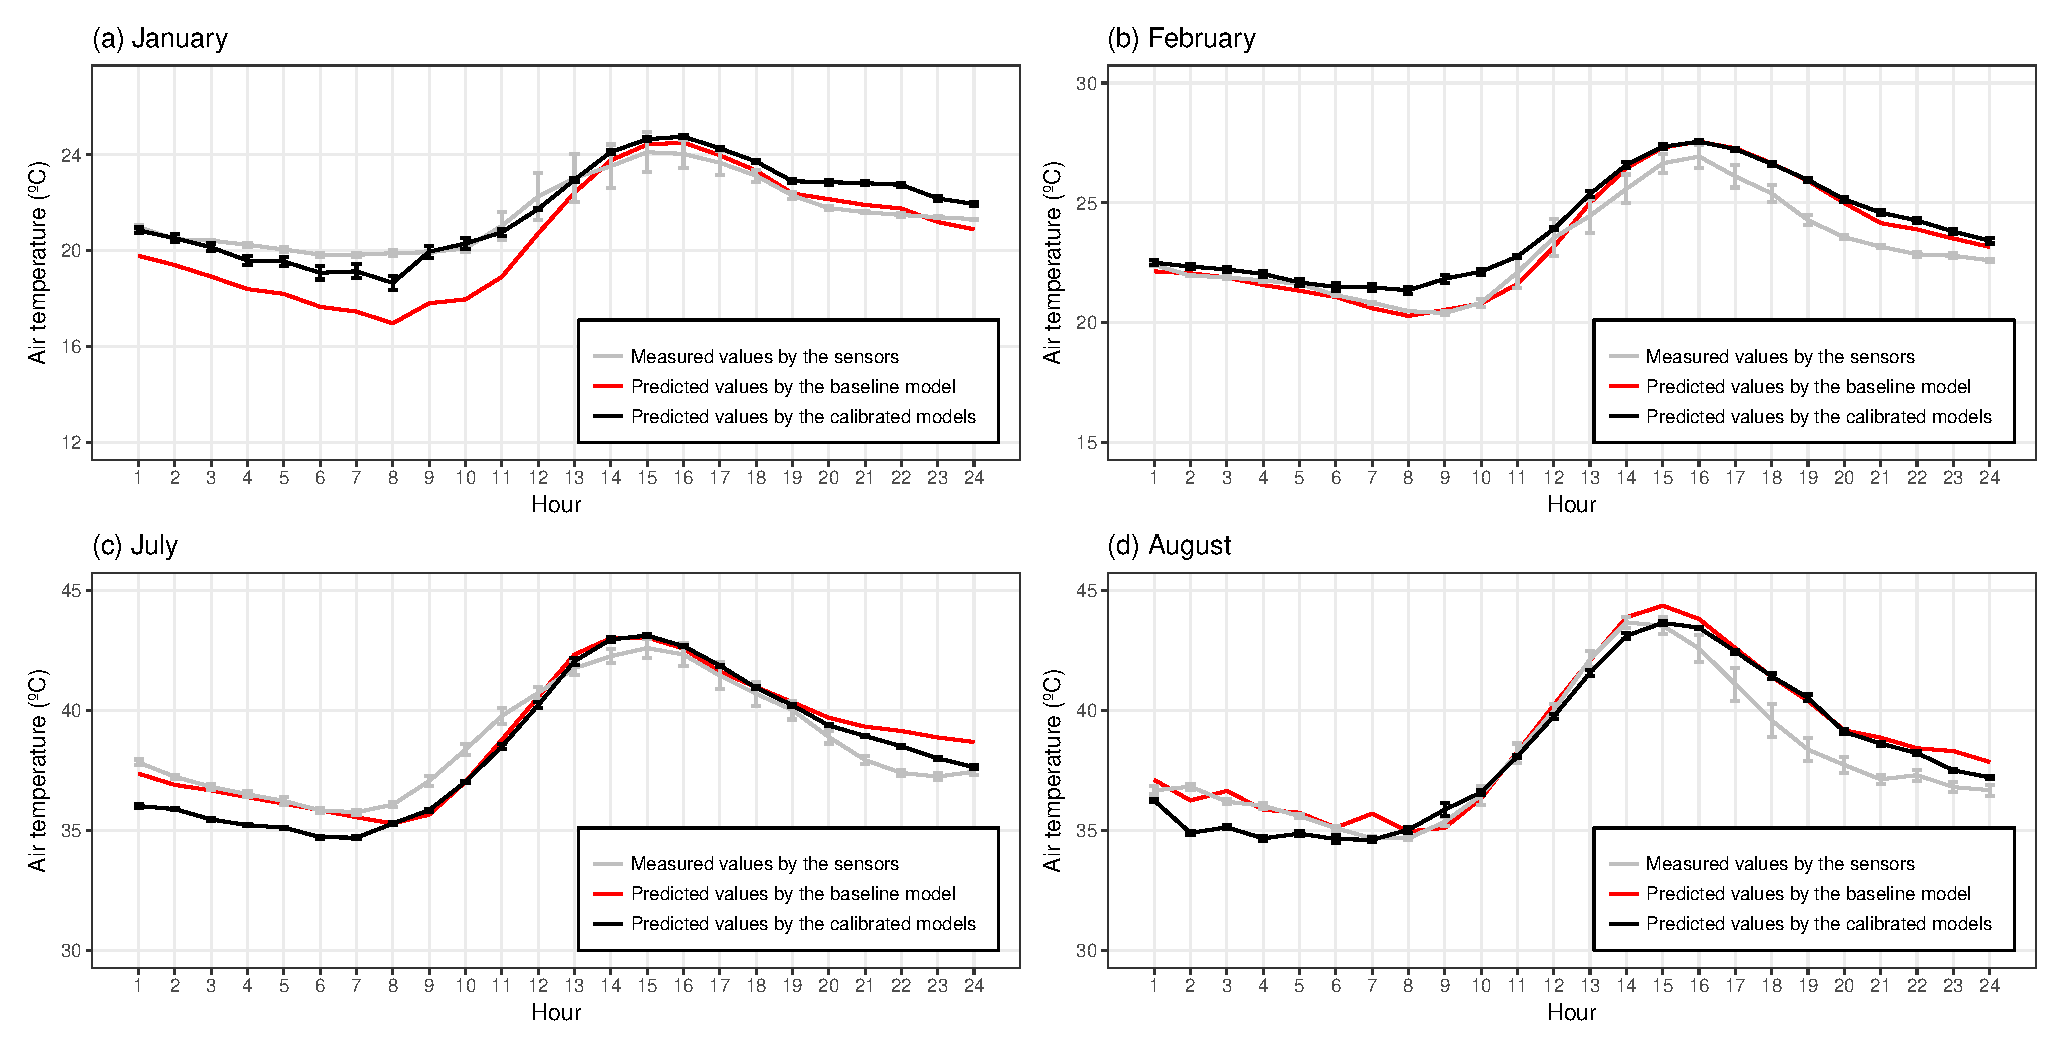
\includegraphics[width=\linewidth]{Figure5-5.eps}
\caption{Weekly-average diurnal profiles of the urban outdoor air temperature: (a) Data between January 15 and 21, 2017; (b) Data between February 8 and 14, 2017; (c) Data between July 15 and 21, 2017; (d) Data between August 8 and 14, 2017. The error bar represents one standard deviation of the measured values by the sensors and the predicted values by the 10 calibrated models, respectively. The baseline model has been manually calibrated via detailed investigations.}
\end{figure}

\begin{table}[]
\footnotesize
\begin{center}
\caption{Performance of the baseline and calibrated UWG models based on two weekly-average diurnal profiles of the urban-rural outdoor air temperature difference.}
\makebox[\linewidth]{
\begin{tabular}{llll}
\toprule
\textbf{Scenario}                                                 & \textbf{January 15-21}                          \\ \hline
Evaluation metric                                        & NMBE          & CV(RMSE) & GOF           \\ \hline
Measured values \textit{v.s.} predicted values (baseline model)   & -0.27         & 0.43     & 0.29          \\
Measured values \textit{v.s.} predicted values (calibrated model) & 0.05          & 0.21     & \textbf{0.08} \\ \hline
\rule{0pt}{2.75ex}\textbf{Scenario}                                                 & \textbf{February 8-14}                          \\ \hline
Evaluation metric                                        & NMBE          & CV(RMSE) & GOF           \\ \hline
Measured values \textit{v.s.} predicted values (baseline model)   & 0.36          & 0.69     & \textbf{0.40}  \\
Measured values \textit{v.s.} predicted values (calibrated model) & 0.77          & 0.90      & 0.78          \\ \hline
\rule{0pt}{2.75ex}\textbf{Scenario}                                                 & \textbf{July 15-21}                             \\ \hline
Evaluation metric                                        & NMBE          & CV(RMSE) & GOF           \\ \hline
Measured values \textit{v.s.} predicted values (baseline model)   & 0.18          & 1.06     & \textbf{0.38} \\
Measured values \textit{v.s.} predicted values (calibrated model) & -0.41         & 1.22     & 0.55          \\ \hline
\rule{0pt}{2.75ex}\textbf{Scenario}                                                 & \textbf{August 8-14}                            \\ \hline
Evaluation metric                                        & NMBE          & CV(RMSE) & GOF           \\ \hline
Measured values \textit{v.s.} predicted values (baseline model)   & 0.57          & 0.87     & 0.61          \\
Measured values \textit{v.s.} predicted values (calibrated model) & 0.17          & 0.89     & \textbf{0.33} \\
\bottomrule
\end{tabular}
}
\end{center}
Note: For the measured values by the sensors and predicted values by the calibrated models, we use the average to evaluate the performance. The bold type highlights which model performs better in terms of the GOF for each scenario. The baseline model has been manually calibrated via detailed investigations.
\end{table}

Overall, the calibrated solutions (black curve) produce weekly-average diurnal profiles of the urban outdoor air temperature similar to the baseline solution (red curve), as shown in \textbf{Figure 5-5}. Sometimes the calibrated models represent the observed behavior better than the baseline model (e.g., January). This is very encouraging since the baseline model has been manually refined and calibrated for over one year via exhaustive investigations of the local construction documents, regular on-site visits, and detailed discussions with experienced engineers and building management personnel. In addition to the performance guarantee from the calibrated models, one great advantage of the methodology proposed in this study lies in the time consumed to obtain them. For this case study, a total of only $\sim$1000 simulations (which take at most two days without parallel computing) on average have resulted in an improved urban microclimate model. So, it seems highly cost-effective and convenient to use the developed algorithm in the process of model calibration.

A further consideration of the hourly data is shown in \textbf{Figure 5-6}, where four days in each validation period are depicted. In general, the calibrated solutions are able to capture most trends as well as peaks and valleys of the measurements. This is impressive because in this study we calibrated the model parameters for a whole year based on just two weekly-average diurnal profiles of the urban-rural outdoor air temperature difference. More data with higher spatial and temporal resolution are being collected and it is reasonable to expect that, if these data were used to calibrate the model, the resulting solutions could achieve higher accuracies with lower uncertainties. Whether the improved performance is commensurate with the extra resources and efforts required to perform accurate measurement and conduct optimization-aided calibration on urban-scale models is not clear and should be investigated in the future.

\begin{figure}[!h]
\centering
\includegraphics[width=.95\linewidth]{Figure5-6.eps}
\caption{Hourly diurnal profiles of the urban outdoor air temperature in 2017. The solid line represents the average of the measured values by the sensors and the predicted values by the 10 calibrated models, respectively. The shaded area represents one standard deviation of the measured values by the sensors and the predicted values by the 10 calibrated models, respectively. The baseline model has been manually calibrated via detailed investigations.}
\end{figure}

Finally, one particular aspect to notice in \textbf{Figure 5-6} is the unexpected behavior during July 17-18, where large discrepancies between predicted and measured data are evident. A good fit to the weekly-average diurnal profile (i.e., the one with low GOF shown in \textbf{Figure 5-5}) may not necessarily predict the hourly diurnal profile more accurately. One possible reason is that, there may be some short-term physical activities (e.g., anomalous wind patterns) during that time which can largely affect the corresponding urban microclimate condition, while such physical activities have not been adequately modeled in the current UWG or have not been reflected in the given rural weather data. This strong bias needs to be revisited in our future studies and may call into question a conclusion from a previous UWG assessment that the location of the reference station has minimal impact on the estimate of temperatures at district level because the urban-canopy energy balance is weakly influenced by advection in the urban boundary layer \cite{bueno2014computationally}. Nevertheless, in most cases, the differences are quite acceptable given the state of the art of urban microclimate modeling.



